\documentclass{article}

\usepackage[utf8]{inputenc}

\usepackage{amsmath, bm}
\usepackage{graphicx}
\usepackage{amssymb}
\usepackage{float}
\usepackage{caption}
\usepackage{subcaption}
\usepackage{hyperref}
\usepackage{tikz}
\usepackage{layout}
\usepackage{wrapfig}

\usepackage[margin=1in]{geometry}
\usepackage{listings}
\usepackage{xcolor}
\usepackage{color, colortbl}
\usepackage{textgreek}
\usepackage{mathrsfs}
\usepackage{savetrees}

% 12 pt font
\renewcommand{\normalsize}{\fontsize{12pt}{\baselineskip}\selectfont}

\begin{document}

\title{4A7 Transonic Wing Design}
\author{lwp26}
\date{May 2024}
\maketitle

\section{Introduction}


The development of high-efficiency transonic aerofoils, can significantly improve the overall performance of an aircraft.
The Breguet range equation, which calculates the range of an aircraft, directly depends on the flight speed and lift to drag ratio of the wing:

\begin{equation}
S = \frac{U}{g}\frac{L/D}{\text{sfc}} \log \left( \frac{W_\text{start}}{W_\text{end}} \right)
\end{equation}

where $S$ is the range, $U$ is the flight velocity, $g$ is the acceleration due to gravity, $\text{sfc}$ is the specific fuel consumption of the engine, and $W_\text{start}$ and $W_\text{end}$ are the initial and final weights of the aircraft, respectively.
This shows increasing flight speed and lift to drag ratio will increase the range of the aircraft.
In the troposphere where temperature decreases, maximising range is equivalent to maximising $M \cdot L/D$.

Previous work in subsonic aerofoil design maximising $L/D$ showed the importance of the boundary layer growth on the viscous drag of the wing.
Adjustments were made to surface curvature, changing pressure gradients in effort to delay transition and separation, minimising boundary layer growth \cite{SA1_report}.
Transonic aerofoil design is more complex than subsonic design due to the formation of shock waves on the wing surface.
Additional lift is obtained by maximising suction peak and area of supersonic flow, however there is an additional source of wave drag that increases with shock strength.
The general goal of our design process therefore was to delay the position and strength of the shock wave.
However, this location and strength were observed to be highly sensitive to the geometry, which is likely due to small changes to Prantle Meyer
expansion fan angles causing large changes in the position of reflected compression lines from the constant pressure boundary.
These expansion angles are also dependent on local geometry and local Mach number, causing a chaotic design space.

The chosen operating point for the design was $M=0.75$, $\alpha = 2.3^\circ$ and $Re=10^6$.
 
\section{Design Process}

The final design and surface curvature plots are shown in figure \ref{fig:airfoil}, while the pressure coefficient distribution at operating point is shown in figure \ref{fig:cp_vs_xc}.
High curvature at the leading edge provides rapid expansion to the suction peak, maximising lift here.
The first spline point had to be moved down to ensure that theres no inflection point on the upper surface due to centerline spline and thickness distribution.
A very small amount of curvature is maintained around the top surface to prevent further expansion in the supersonic region,
and to allow the reflected expansion lines to compress the flow, reducing the shock strength.
Flatter and concave curvatures at mid-chord of the upper surface were tested but these increased curvature at the trailing edge, increasing back pressure which caused two shocks to form.
This region of increased curvature is required to return to the surface back to the trailing edge.
At the end of the upper surface, there is some concave geometry where the upper and lower pressure distributions cross over.
This causes downforce, which is poor for lift and comes as a result of the thickness distribution.

\begin{figure}[H]
    \centering
    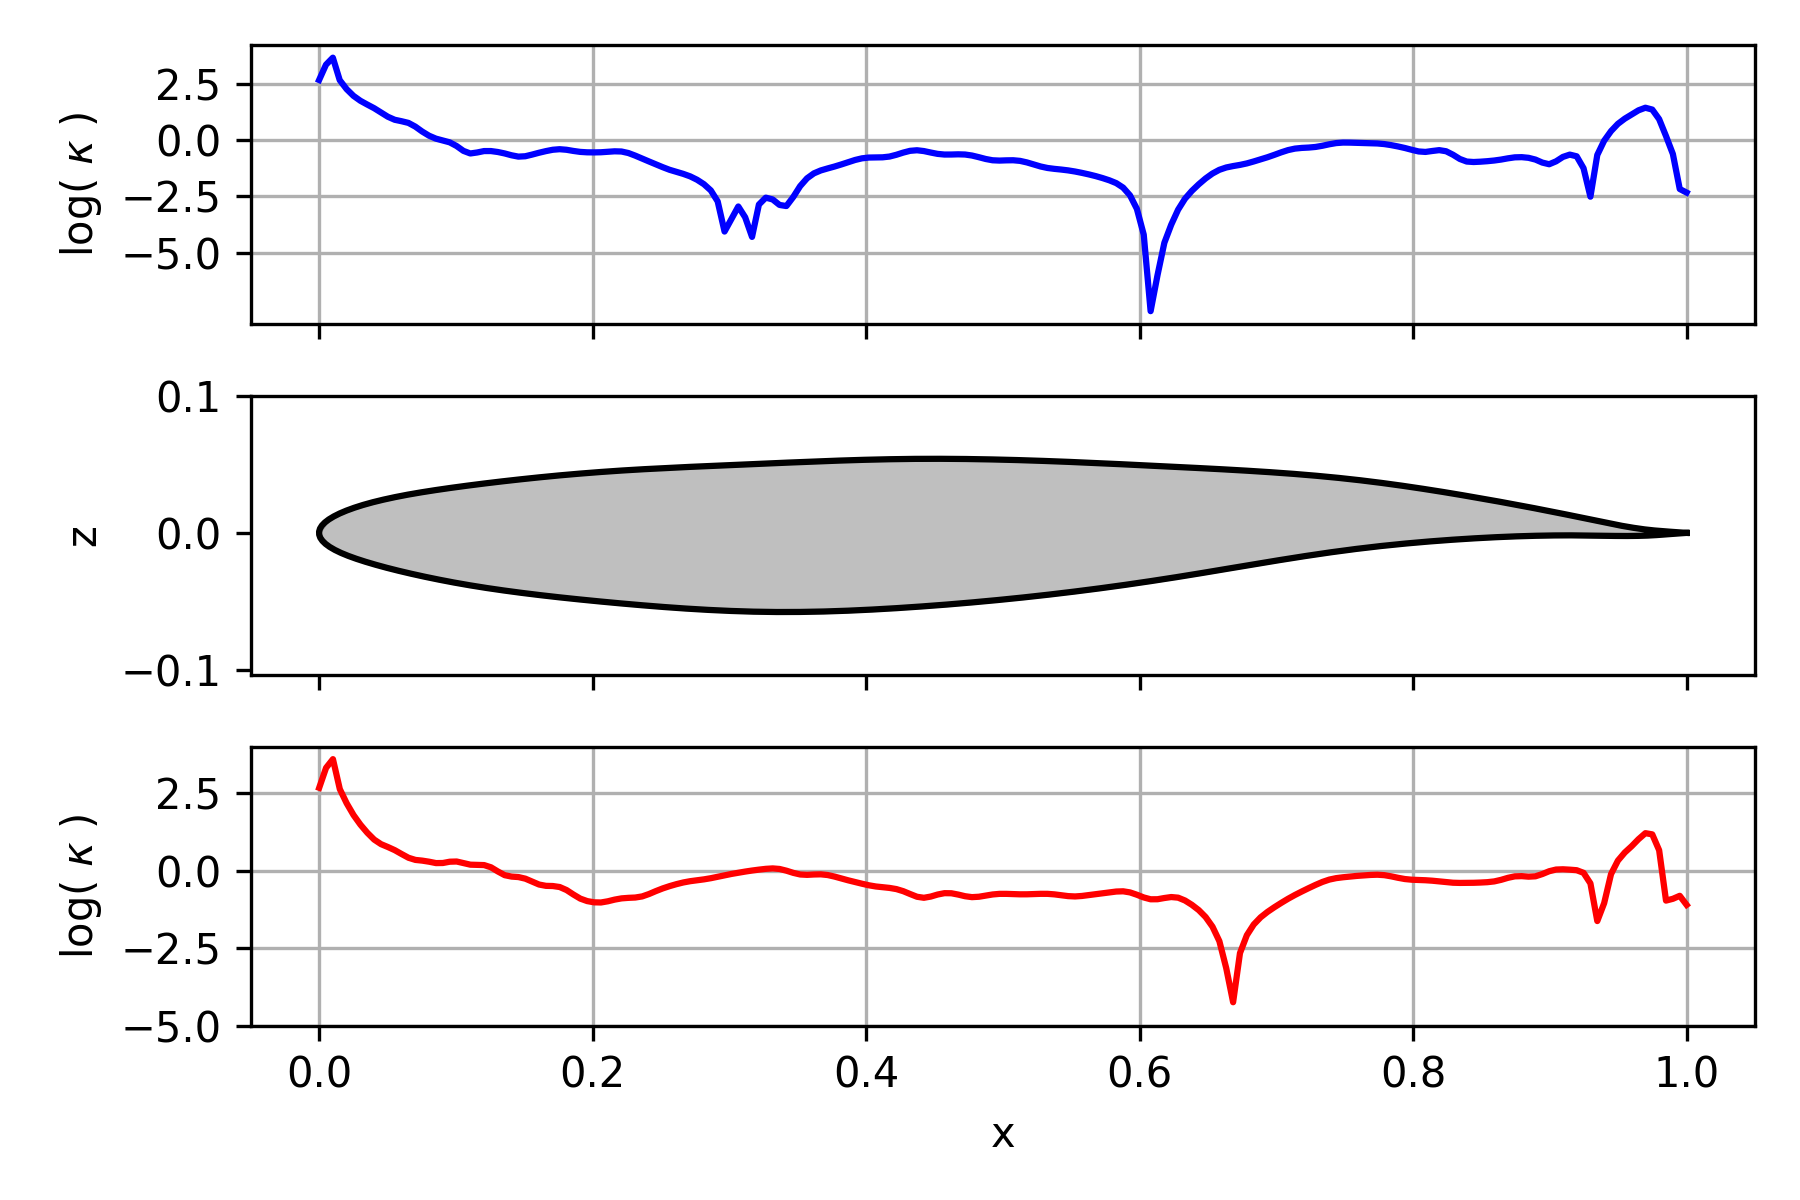
\includegraphics[width=0.7\textwidth]{figures/airfoil.png}
    \caption{Aerofoil cross-section}
    \label{fig:airfoil}
\end{figure}

\section{Improvements}
% Which features of the design are you not happy with and how could it be improved further
% given more time/effort (i.e. what would your ideal design c p distribution look like)? Which
% negative features are unlikely to be ‘fixable’?
Examples of target upper $C_p$ distributions are shown in reference \cite{esdu} and consist of one with no shock, and one with a weak shock.
These typically consist of a region of rapid acceleration over 3\% of the chord, followed by a small smooth rounded peak to a long linear region of gradual compression.
The section behind has a much greater rate of compression by weak shock or compression fan.
Results from the program VGKD where geometry is optimised to closely match target upper surface pressure distributions demonstrate this is feasible.
The pressure distribution achieved by our design differs from this ideal in the nonlinear compression region, and has earlier and stronger shock formation.
Off design point, the adverse pressure gradients in the nonlinear compression region form shocks, then reaccelerate the flow in the favourable pressure gradient region and shock again.
This can be fixed by reducing curvate at these locations but may require a more sensitive change in spline control points.
Fine control of the curvature could also likely delay the shock formation and reduce its strength by allowing more reflected compression lines to take effect.
The crossover at trailing edge could also be improved with an antisymmetric thickness distribution, which may not be feasible in VGK
but regardless is a limitation of the software as this cannot be changed without re-selecting a new thickness distribution.
Crossover is also observed in many designs produced by VGKD \cite{esdu}.

\section{Limitations}

\begin{itemize}
    \item  The software is only valid for 2D infinite length wings which neglects the effects of downwash due to wing tip vortices and other 3D flow effects.
    \item  VGK uses the Lag-Entrainment integral method for turbulent boundary layers which relies on empirical correlations
and poorly models some shock boundary layer interactions \cite{lagentrainment}.
    \item  Doubts about the accuracy of the VGK solver arise when the boundary layer on the upper or lower surface is close to separation \cite{esdu}.
    \item  Numerical errors can also arise from the discretisation of the geometry and the flow field.
    \item Cases where the VGK software fails to converge are not included in the data set and the cause of these failures may be unsteady buffeting or general impractical flow conditions.
    \item A limitation with the front end software, mentioned earlier, is the lack of an antisymmetric thickness distribution.
\end{itemize}

It is also important to note that the performance of designs produced by the VGK software can be extremely sensitive
within even the small manufacturing tolerances in the aerospace industry.
Additional practical design requirements could be for structural reasons or volumetric fuel capacity.

% reference SA1 wing analysis report

\begin{figure}
    \centering
    \begin{subfigure}[t]{0.45\textwidth}
        \centering
        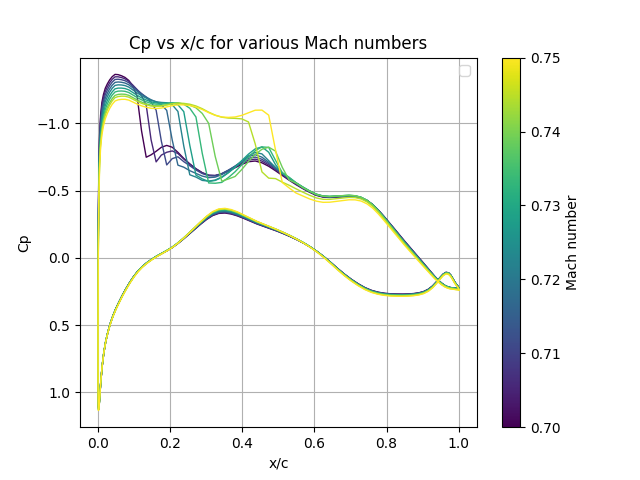
\includegraphics[width=\textwidth]{figures/cp_vs_xc_machs.png}
        \caption{Pressure coefficient distribution at $M=0.75$, $\alpha = 2.3^\circ$.}
        \label{fig:cp_vs_xc}
    \end{subfigure}
    \begin{subfigure}[t]{0.45\textwidth}
        \centering
        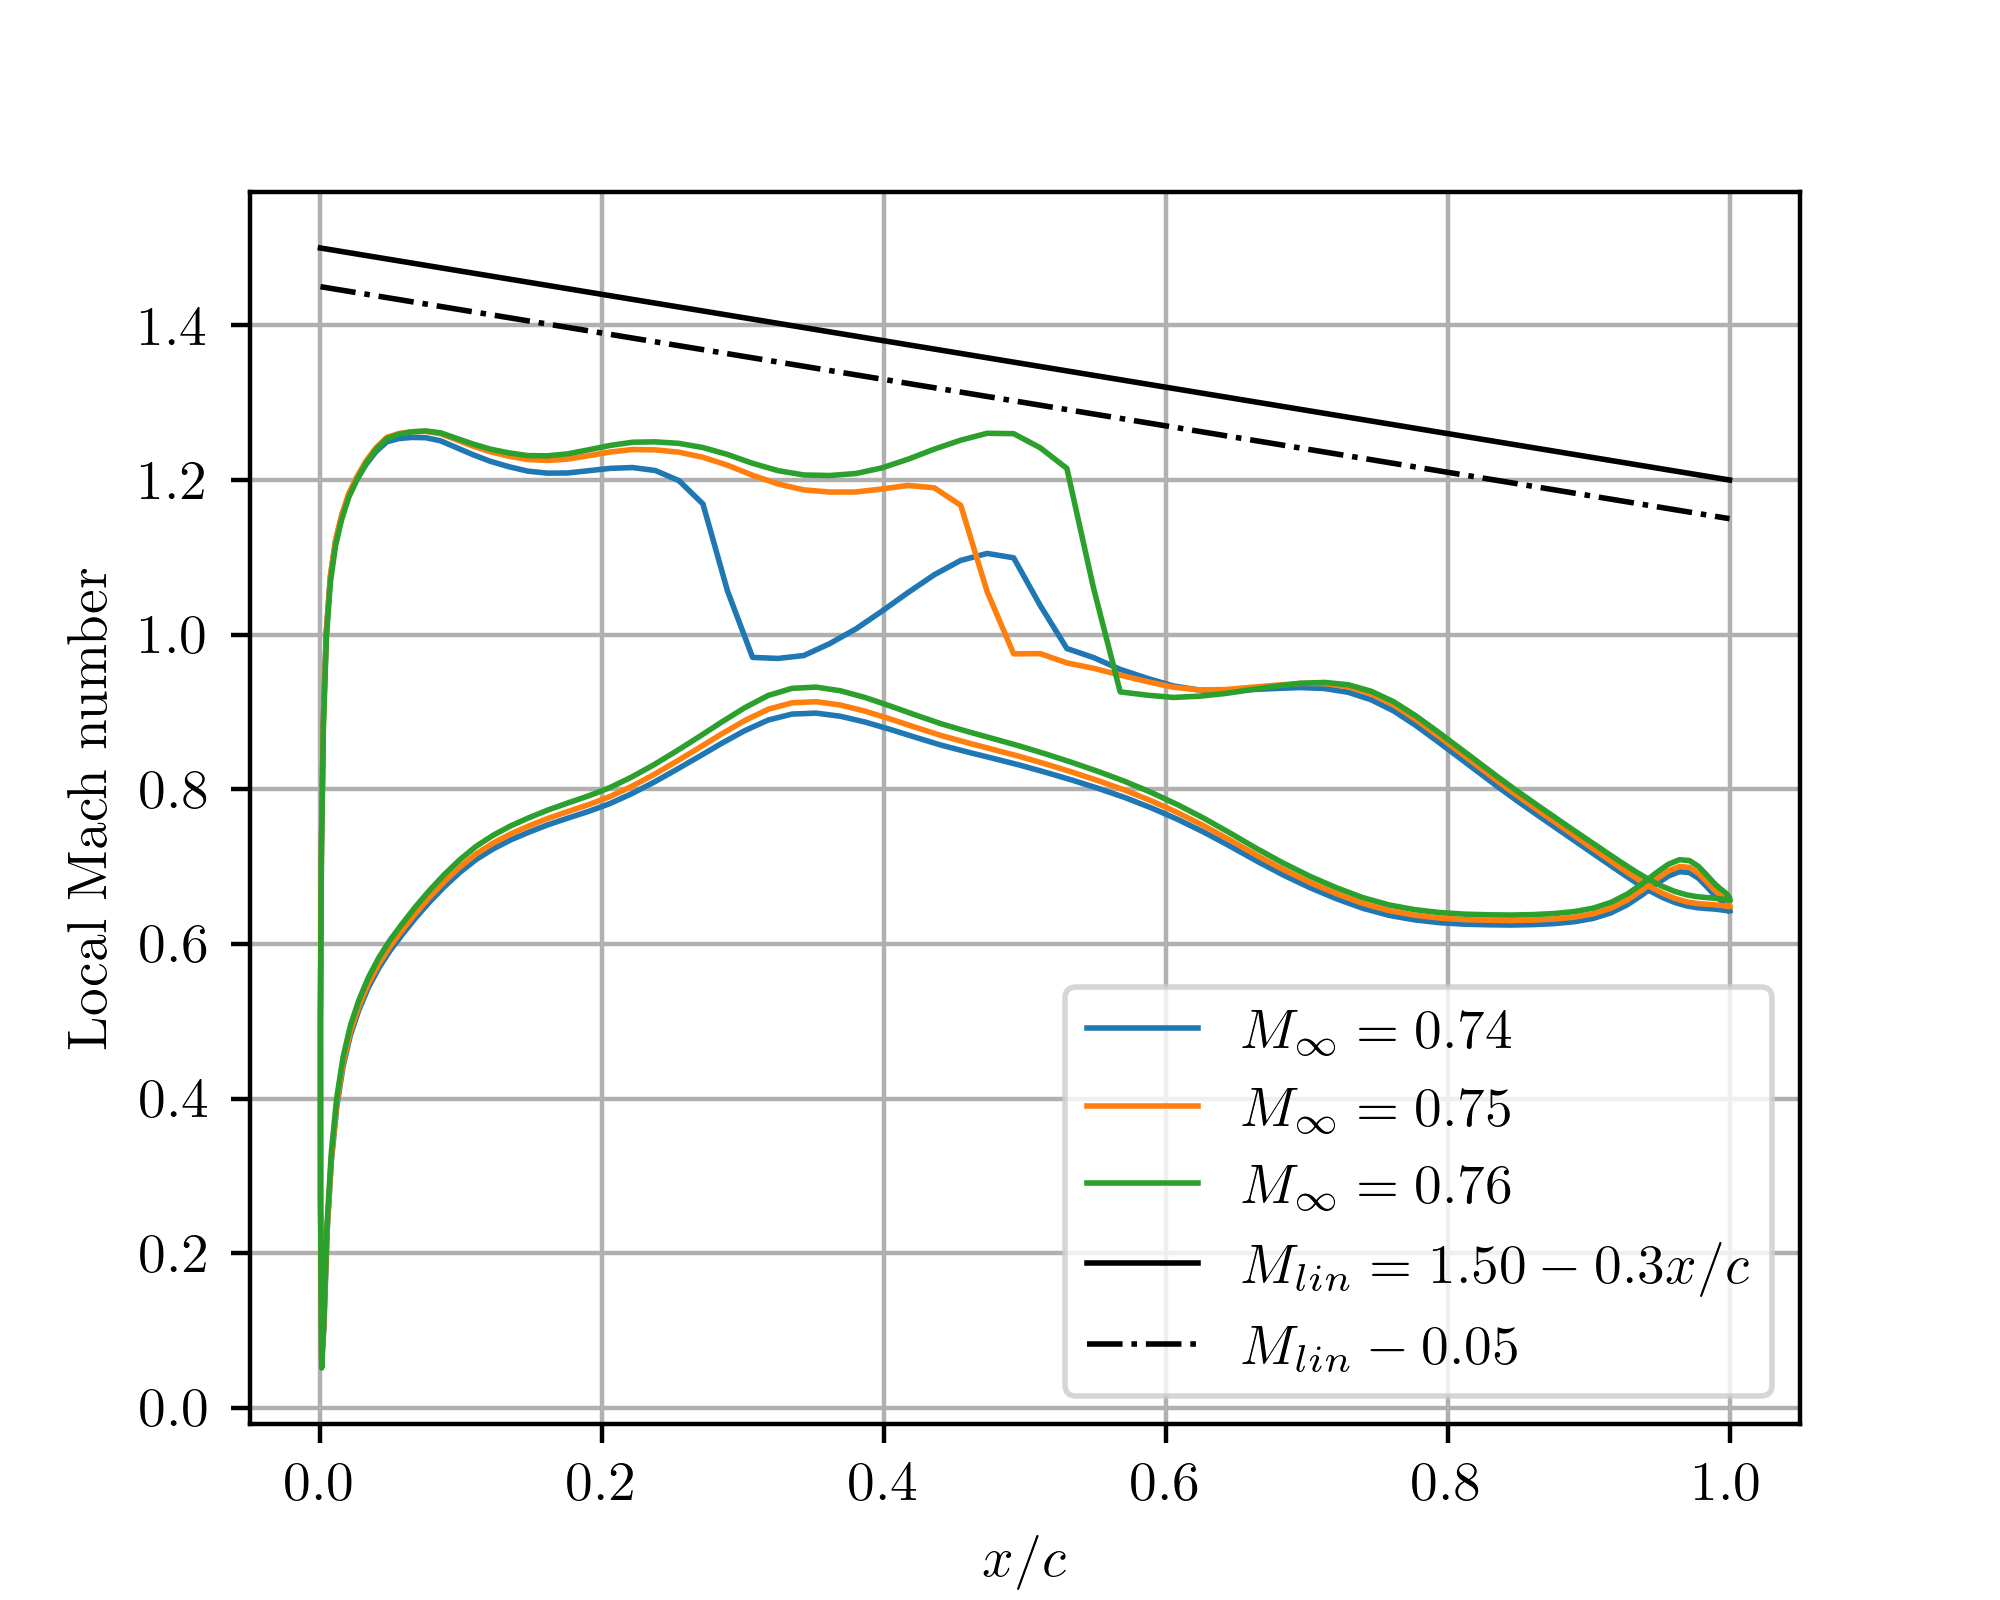
\includegraphics[width=\textwidth]{figures/mach_vs_xc.png}
        \caption{Mach number distribution at various $M_\infty$ and $\alpha = 2.3^\circ$}
        \label{fig:mach_vs_xc}
    \end{subfigure}
    \caption{}
\end{figure}

\begin{figure}
    \centering
    \begin{subfigure}[t]{0.45\textwidth}
        \centering
        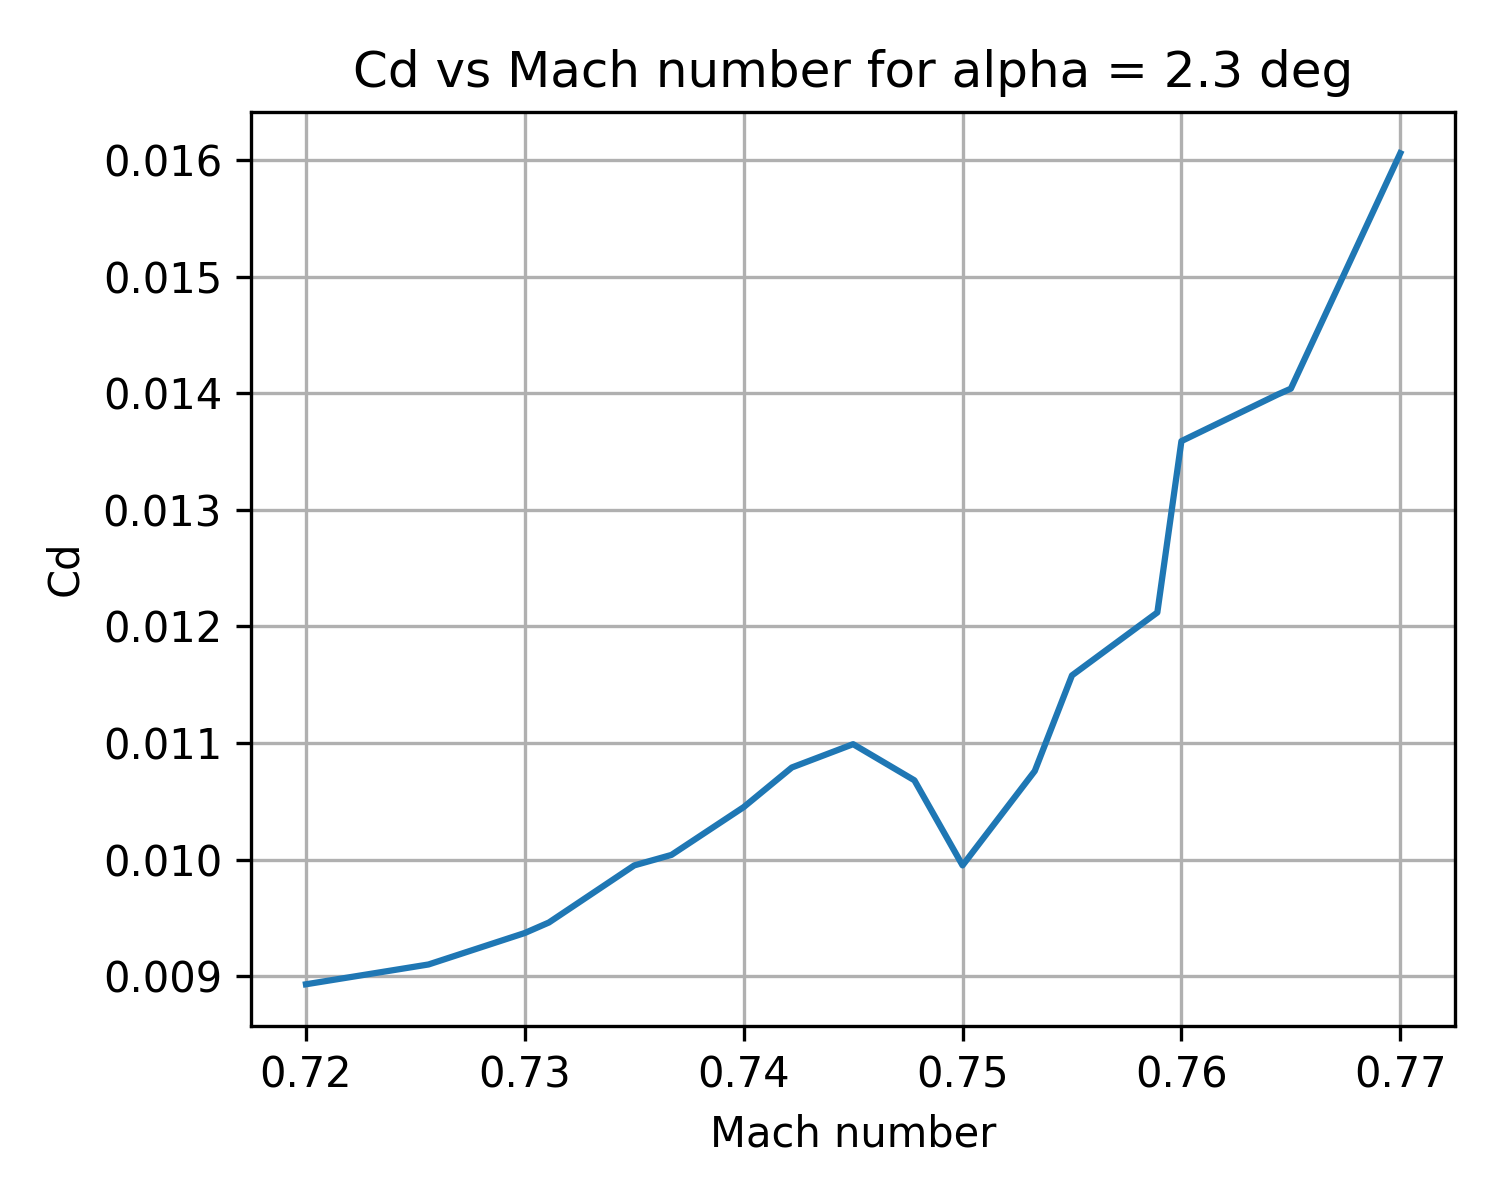
\includegraphics[width=\textwidth]{figures/cd_vs_mach.png}
        \caption{Drag coefficient vs Mach number}
        \label{fig:cd_vs_mach}
    \end{subfigure}
    \begin{subfigure}[t]{0.45\textwidth}
        \centering
        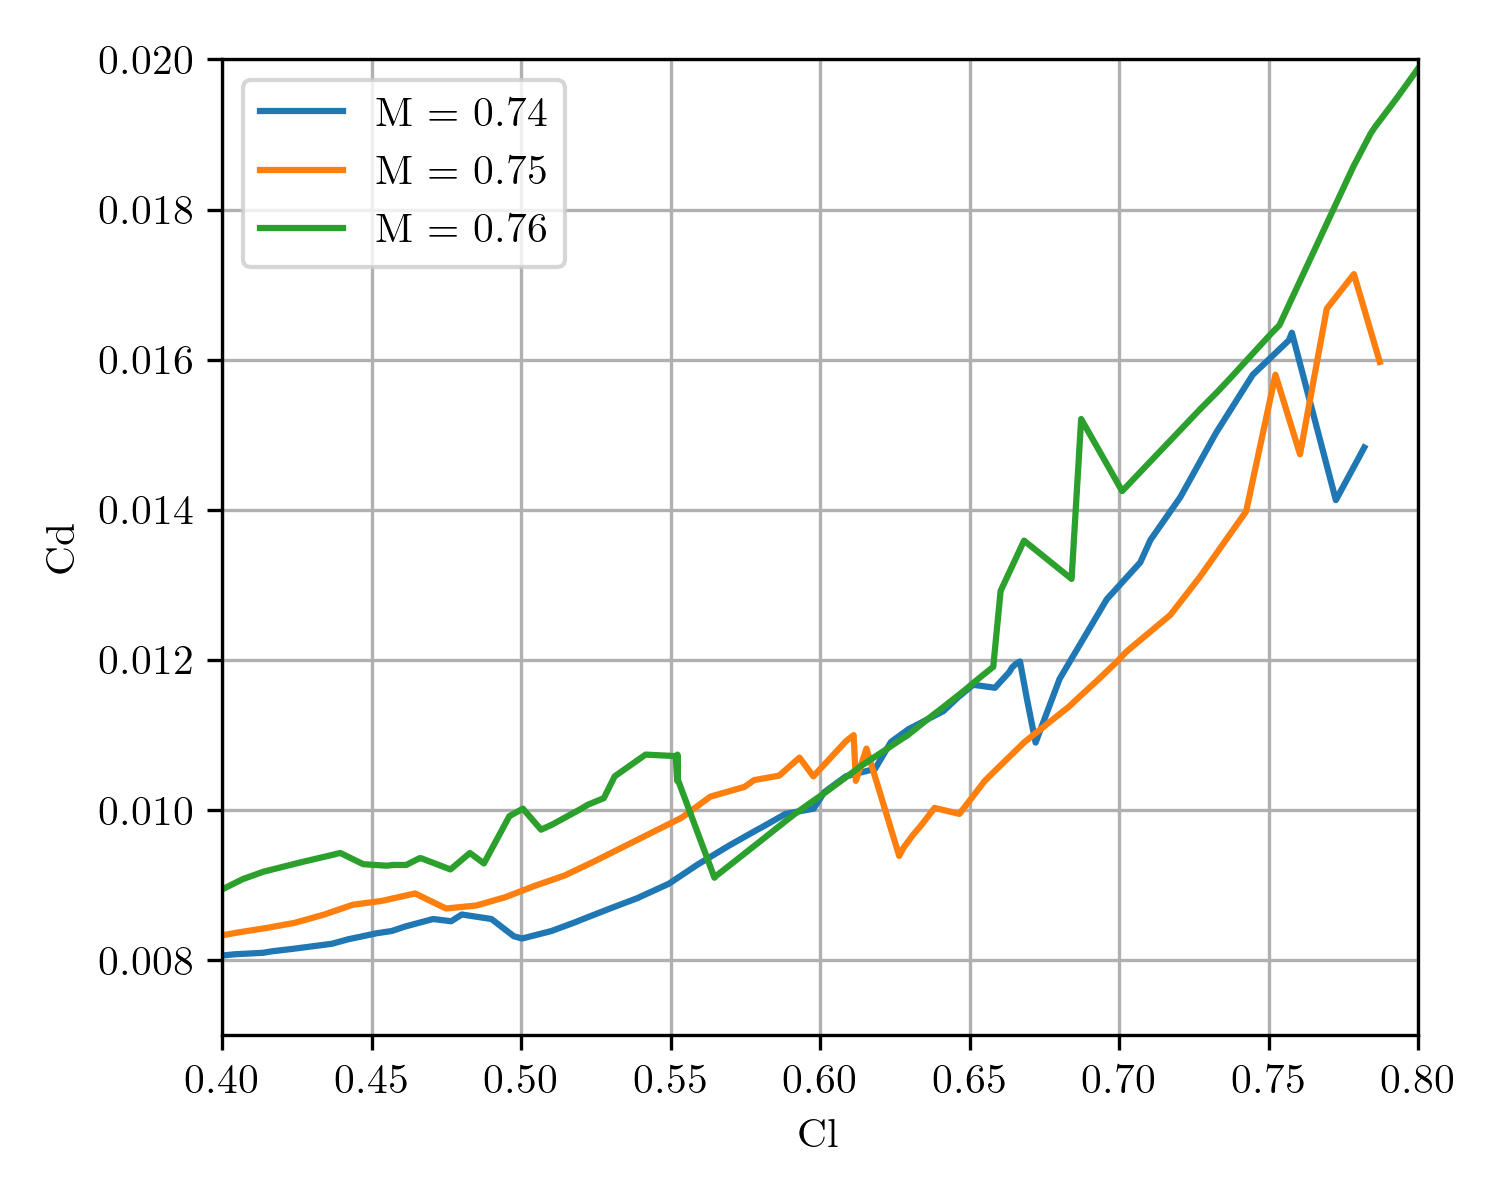
\includegraphics[width=\textwidth]{figures/cd_vs_cl.png}
        \caption{Pressure coefficient distribution for different Mach numbers}
        \label{fig:cd_vs_cl}
    \end{subfigure}
\end{figure}

\newpage

\section{Buffet Line}

Buffet is complex unstable interaction between the shockwaves and boundary layers and can produce large amplitude pressure fluctuations on the wing surface.
This can be damaging to the aircraft structure and cause a loss of control.

There are various measures to detect the onset of buffet
\begin{itemize}
    \item Shock entry Mach number, taken at shock of maximum strength
    \item Trailing edge shape factor, $\overline{H}_{te}$
    \item High Mach numbers close to trailing edge, measured by a minimum distance between Mach distribution and line $M_{lin}$.
    \item Trailing edge pressure coefficient rise of 0.04 above its plateau value.
\end{itemize}
These are quantified in the non-dimensional buffet factors, seen on Figure \ref{fig:buffet_classification}.
The data consists of 4684 converged solutions at different Mach numbers and angles of attack which were automatically collected and saved using a Python script.
These points are used to interpolate a 2D gridspace, which is then smoothed using a Gaussian filter, and a buffet contour is drawn at 0.

The first factor shown in figure \ref{fig:buffet_classification}a is a first indication that the shock is strong enough to cause buffet.
This shows that in many operating points of high Mach number and lift coefficient, the shock is strong enough to cause buffet.
The line shows a wave like shape with unusually strong shocks at low Mach numbers.
This was found to be due to a stronger shock occuring earlier due to what is thought to due to a larger constant pressure boundary
reducing the compressive effect of the reflected expansion lines.
The locations of these shocks were typically behind bumps of adverse pressure gradients, as seen in figure \ref{fig:mach_vs_xc}.

The second factor in figure \ref{fig:buffet_classification}b offers an indication of trailing edge separation, which can relieve the shock backpressure, causing buffeting [?].
The trailing edge shape factor at high angle of attack and Mach number combinations passes the threshold of 2.2, indicating a high likelihood of buffet.
Increased shock strength, and more severe adverse pressure gradients can cause boundary layer growth leading to high trailing edge shape factors.
Accuracy of the solver at higher shape factors is also questionable as the solver is not valid for separated flows \cite{esdu}.

\begin{figure}[H]
    \centering
    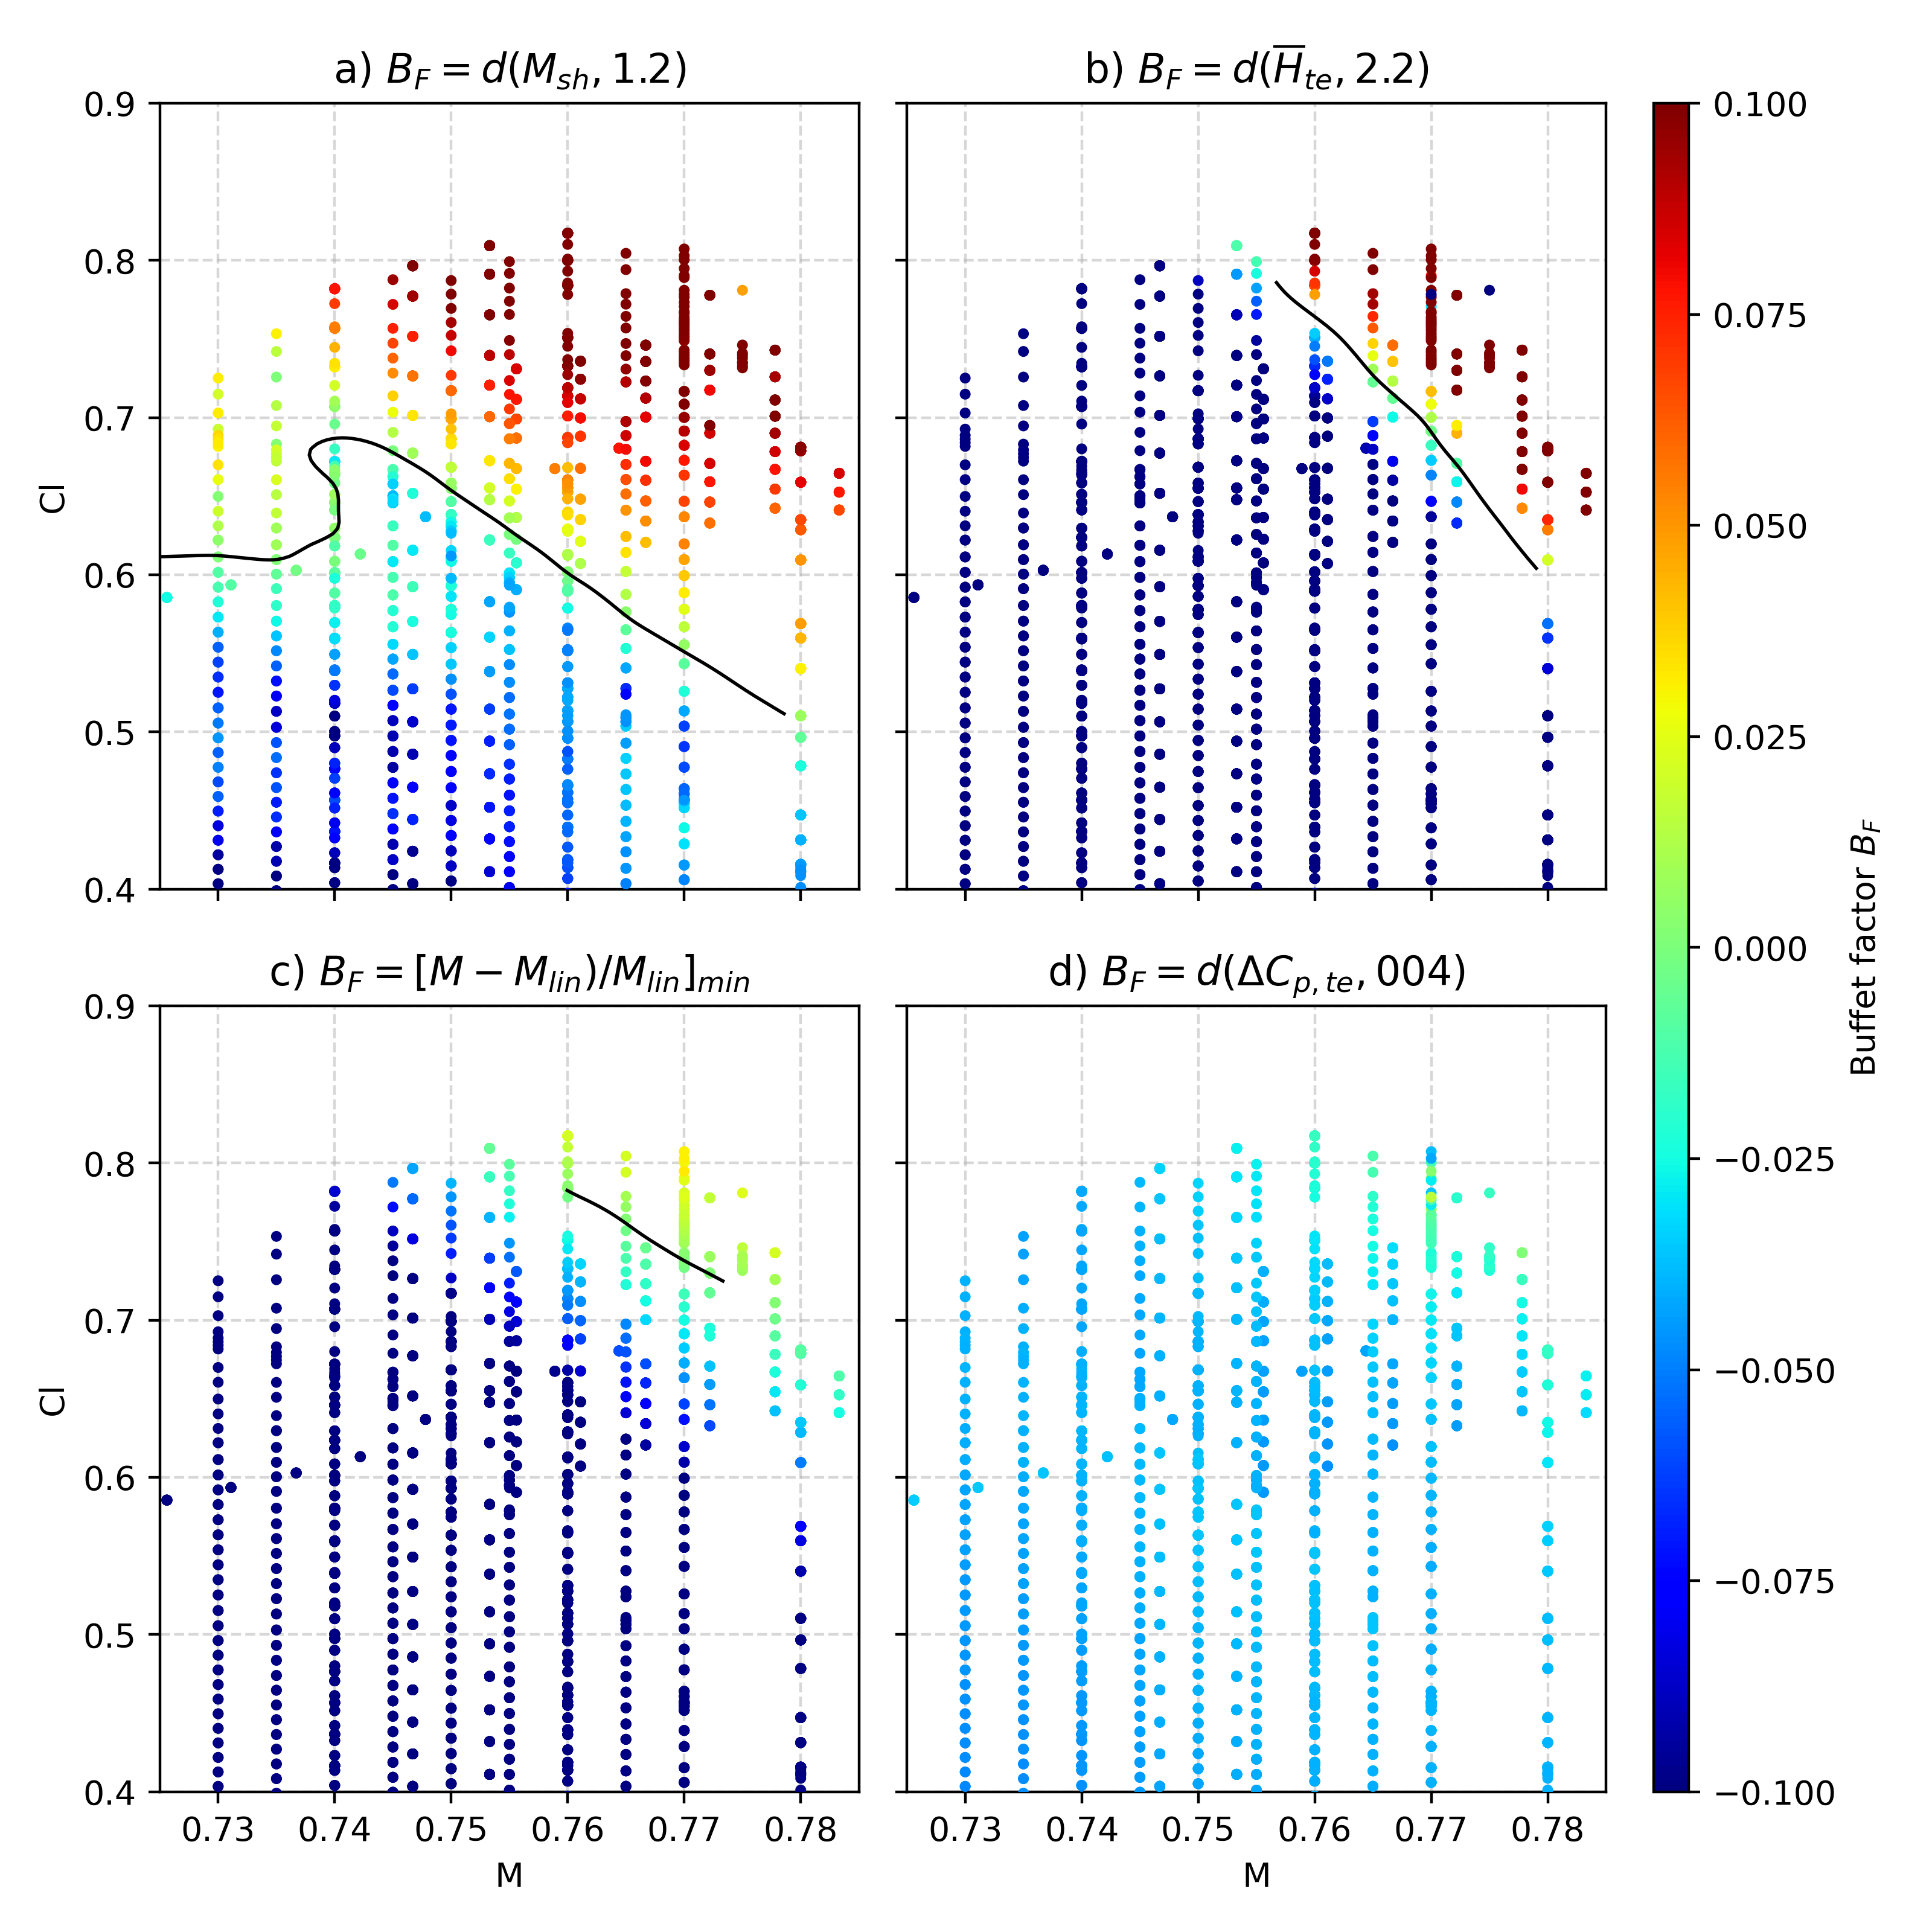
\includegraphics[width=0.8\textwidth]{figures/buffet_classification.png}
    \caption{Buffet factors at a range of Mach numbers and lift coefficients. $d(x,c)$ is the normalised difference $(x-c)/c$}
    \label{fig:buffet_classification}
\end{figure}


The third buffet factor is calculated from the minimim difference between the Mach number plot and linear boundaries shown on figure \ref{fig:mach_vs_xc}.
Figure \ref{fig:buffet_classification}c shows the same lines for the runs with Mach lines that touch the same boundaries.
These show lines with a very similar gradient to that seen in figure \ref{fig:buffet_classification}a but occur at higher Mach numbers and lift coefficients.
It may be that this factor less sensitive to the onset of buffet than the first two, or this indicates that buffet is more severe 

The last factor is the trailing edge pressure coefficient rise above the threshold of 0.04 from its plateau value.
Determining this stable plateau value proved difficult as, although the name suggests its a constant, it actually varied with Mach number.
The plateau was determined at each Mach number by increasing the angle of attack until there is only one shock on the upper surface.
This was due to a sudden drop in trailing edge pressure coefficient when the number of shocks decreased.
A reason for why this happens is not clear.
The factor itself shows a rise at high Mach numbers and lift coefficients, however none of the points in the data set exceeded the threshold and so the contour is not shown.
Many combinations of high Mach numbers and angles of attack were tested but many did not converge, which is likely due to separation occuring.
However, even up until this point the shape factor increases beyond the threshold of 2.2, where doubts about the accuracy of the solver arise \cite{esdu}.

\section{Performance Metric}

\begin{figure}[H]
    \centering
    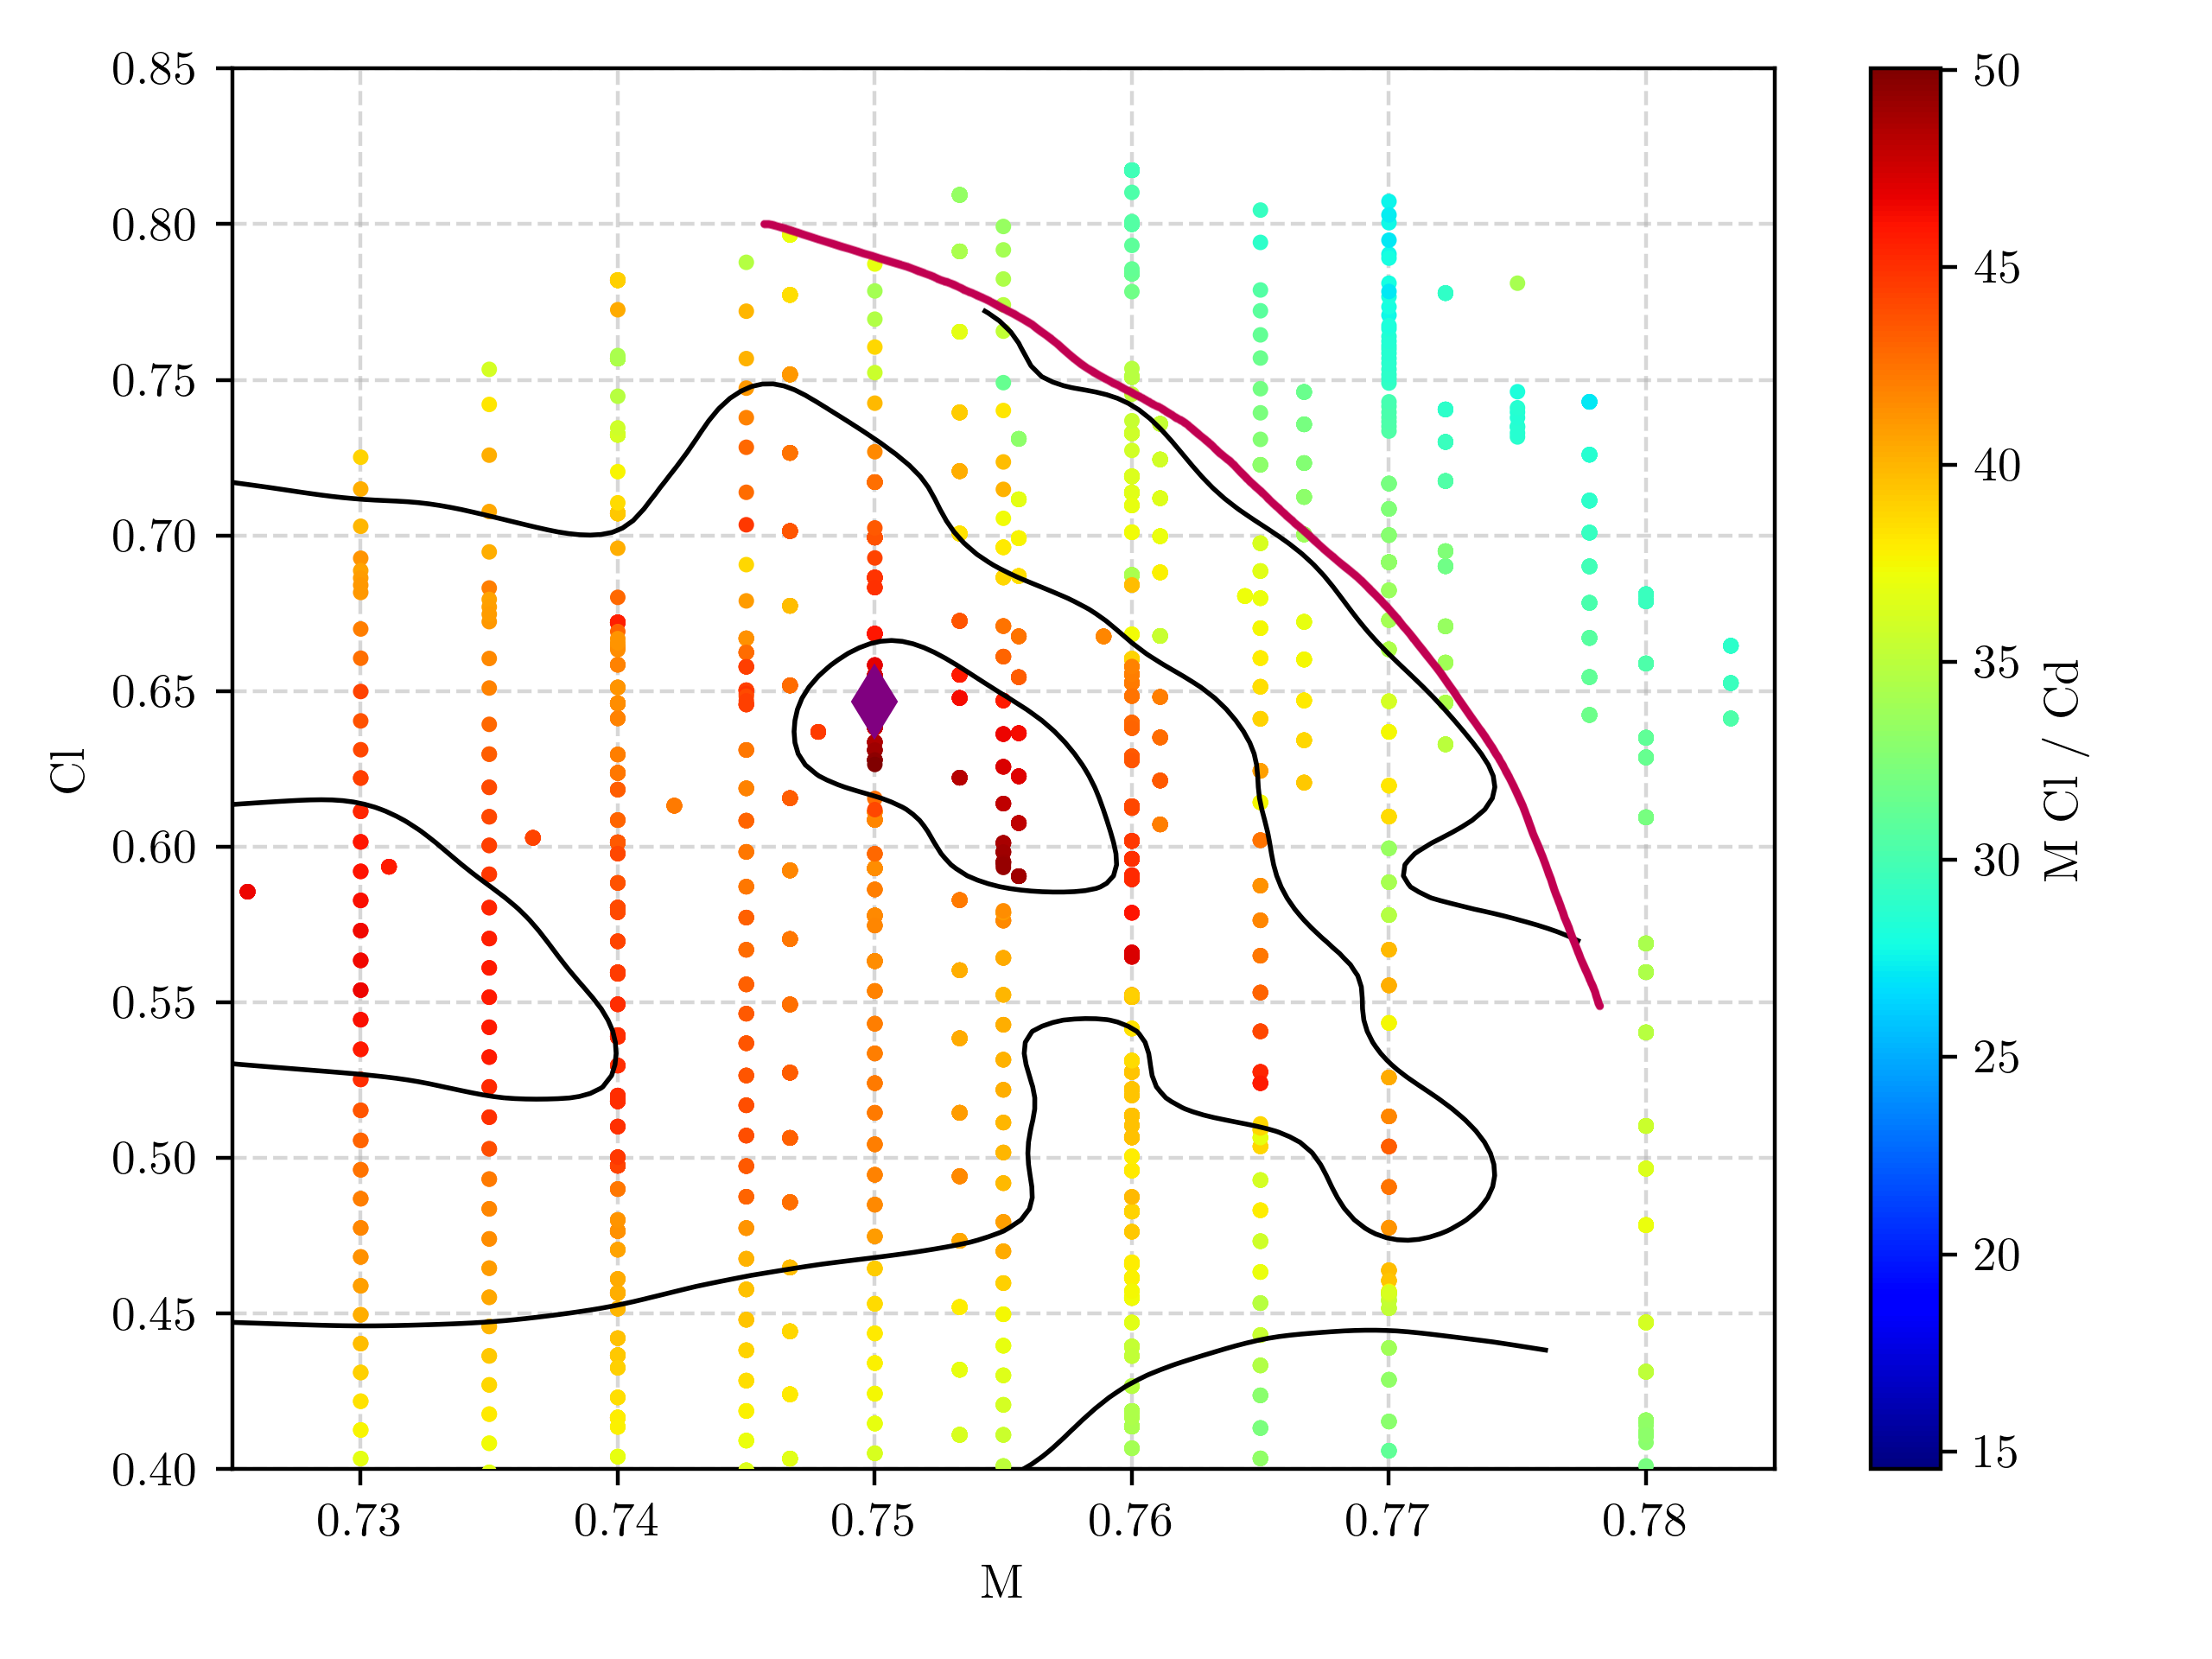
\includegraphics[width=0.7\textwidth]{figures/performance_metric.png}
    \caption{Performance metric and buffet line}
    \label{fig:performance_metric}
\end{figure}

Figure \ref{fig:performance_metric} shows the modified performance metric of $M \cdot C_l/C_d$ and the drawn buffet line.
Its important to note that this is still accurate for swept wings as the Mach number normal to the cross section is multiplied by a constant factor.
The contours show regions of constant performance metric and the buffet line is shown in pink.
Without the $C_d$ term, the graph would have asymptote contours increasing diagonally, however the inclusion of drag
causes a significant drop in performance metric at high Mach numbers and lift coefficients.
One optimal regions for our aerofoil is shown to be close to our design point, with another at slightly lower Mach and angle of attack.
This means we do not necessarily have to lie close to the buffet line to achieve our high performance metric, however some aircraft designers
may prioritise payload capacity, or flight speed over range, and so may choose to operate closer to this line.

The buffet line drawn is a more strict criterion than in \ref{fig:buffet_classification}b, but more relaxed than \ref{fig:buffet_classification}a.
It is recommended that an aircraft designer should not operate in this region and should consider extreme operating conditions.
One such example of an extreme operating condition is a large updraft, increasing the angle of attack and lift coefficient, potentially causing buffet.

\section{Conclusion}

The design process for a transonic wing was discussed, with a focus on modifying upper surface curvature to adjust the shock location and strength.
Comparison with pressure distributions achieved by VGKD showed room for improvement in the compression region and location of the shock.
The limitations of the software were discussed, including the lack of 3D effects and the reliability of the solver to boundary layer separation.
The performance metric analysis and buffet line identification offer practical guidelines for operational safety and efficiency, 
demonstrating that optimal performance does not necessarily require operating near the buffet boundary.
However, extreme conditions, such as updraft-induced increases in angle of attack, highlight the need for robust design margins.

\begin{thebibliography}{9}

      \bibitem{handout}
      J. Jarret
      \emph{4A7 Transonic Wing Design Handout}
      University of Cambridge,
      2024.

      \bibitem{SA1_report}
      L. W. Pender
      \emph{SA1 Wing Analysis Final Report}
      University of Cambridge,
      2024.

      \bibitem{lagentrainment}
      Green J E, Weeks D J and Brooman J W F,
      \emph{Prediction of turbulent boundary-layers and wakes in compressible flow by a lag-entrainment method.}
      ARC

      \bibitem{esdu}
      ESDU 99032
      \emph{VGK Method for Two-Dimensional Aerofoil Sections. Part 5. Design to Specified Upper Surface Distribution}
    
\end{thebibliography}

\end{document}